% !TEX encoding = UTF-8
% !TEX program = pdflatex
% !TEX root = InformationRetrieval.tex
% !TEX spellcheck = it-IT

% 15 Dicembre 2016

\chapter{Anatomia e performance di un sistema di IR}

Nel nostro progetto noi non stiamo misurando lo stemmer di per se, ma stiamo misurando quanto lo stemmer migliora i risultati del sistema rispetto all'esecuzione senza stemming.

Si ha però che il sistema è composto da molti blocchi: tokenizzatore, stoplist, stemmer, modello e quindi non è semplice valutare il singolo componente, perché le prestazioni del sistema possono essere influenzate dagli altri componenti o dai parametri con i quali sono configurati.

Le misure nell'IR sono quindi misure end-to-end che considerano la totalità del sistema. Per valutare un singolo componente stabilisco quindi una pipeline di componenti e vario solamente quello che voglio misurare.

\section{Grid@CLEF}

L'idea è quindi quello di sviluppare un sistema di testing che funzioni con più lingue (MLIA: Multilingual Information Access) per capire come migliorare le performance dei singoli componenti.

Questo si può ottenere conducendo una serie di griglie di esperimenti, sistematici e ripetibili, su diversi linguaggi e con diversi componenti, effettuando uno sforzo comunitario per valutare sia i singoli componenti che la loro interazione con gli altri.

Per implementare questo sistema è stata sviluppata una soluzione asincrona, basata su una produzione di dump intermedi XML, da scambiare tra i vari gruppi di ricerca. Ad esempio quelli che lavoro su un tokenizzatore, possono fornire i loro output ad un gruppi di ricerca che lavora agli stemmer per il tedesco.
Ci sono stati dei problemi implementativi però qualcosa si è riuscito a fare.

\begin{figure}[htbp]
	\centering
	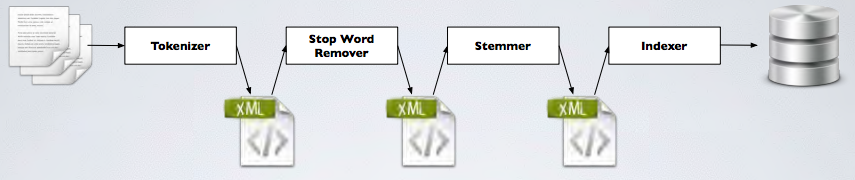
\includegraphics[width=0.5\textwidth]{images/l20-fig-1}
	\caption{Utilizzo dei file XML condivisi dai vari gruppi di ricerca.}
\end{figure} 

Mancava però una metodologia per analizzare i risultati di questi esperimenti.

Nel 2015 alla conferenza SIGIR-RIGOR si è iniziato ad invitare gli sviluppatori di motori open-source a fornire delle baseline di valutazione per i loro sistemi in un ambiente comune.
L'idea era quella di creare questo ambiente comune dove chi volesse valutare una nuova tecnica fosse in grado di utilizzare un motore di ricerca già esistente per il confronto/implementazione. Questo ambiente doveva essere anche aperto in modo che fosse possibile capire se durante i test i sistemi utilizzati fossero stati configurati nella maniera corretta.
Si voleva quindi fornire una baseline da utilizzare come riferimento per i nuovi metodi e allo stesso modo la baseline era in un certo senso certificata perché era nota a tutti e quindi se qualcuno ha presentato dei nuovi modelli comparandoli con una baseline è possibile capire se la baseline di riferimento è sufficientemente buona e quindi i risultati sono concreti, oppure se è stata scelta una baseline pessima e quindi i risultati sembrano migliori di quanto lo sono in realtà.

Ma anche in questo caso mancava una sistema di analisi dei dati.

\begin{figure}[htbp]
	\centering
	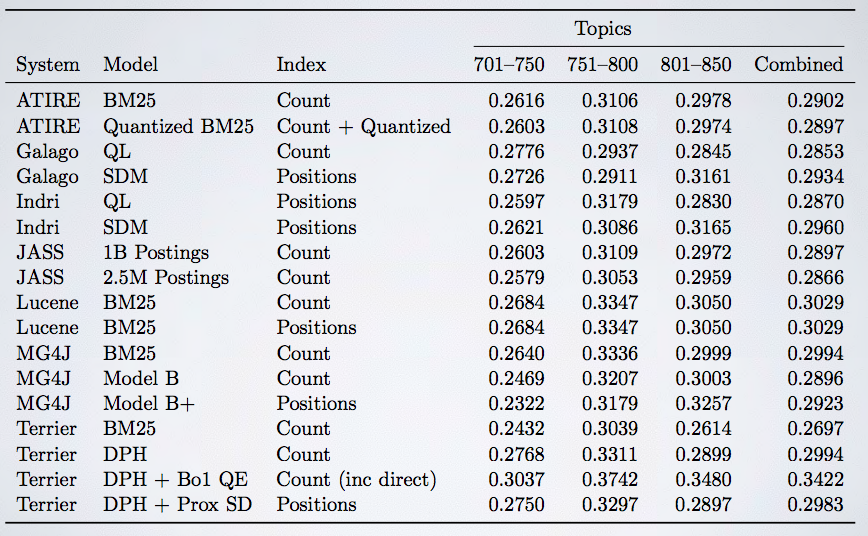
\includegraphics[width=0.5\textwidth]{images/l20-fig-2}
	\caption{Alcuni risultati (Mean Avarage Precision) ottenuti su TREC con il metodo proposto da RIGOR.}
\end{figure} 

\section{Valutazione delle performance - General Linear Mixed Model}

Posso combinare i dati dell'esecuzione dei vari sistemi della griglia in una matrice in cui le righe rappresentano i topic e le colonne sono i vari sistemi. Il valore delle cella è dato dall'average precision del sistema sul dato topic.
La matrice poi può essere plottata in una heat map (figura \ref{fig:heatmap}), in modo che sia più comprensibile.

\begin{figure}[htbp]
	\centering
	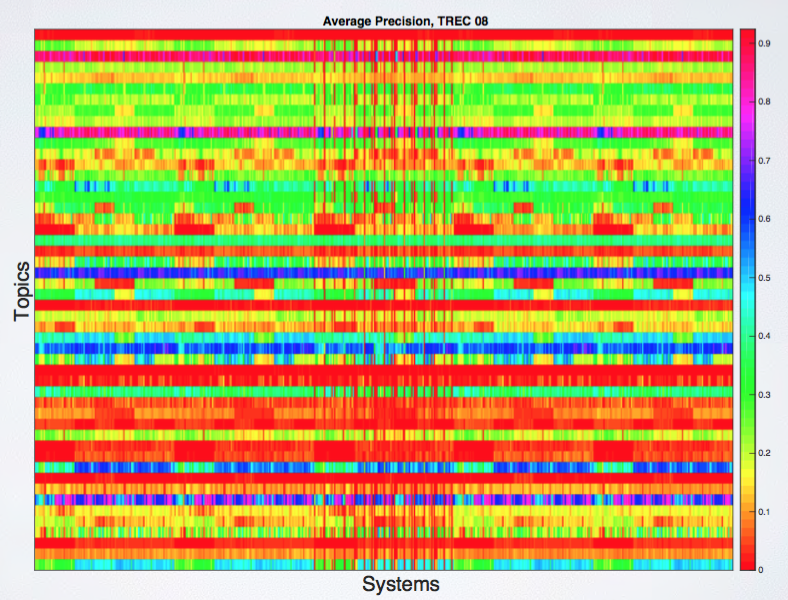
\includegraphics[width=0.5\textwidth]{images/l20-fig-3}
	\caption{Rappresentazione mediante heatmap della matrice. Nelle righe ci sono i topic mentre nelle colonne i vari sistemi.}\label{fig:heatmap}
\end{figure} 

Dalla figura \ref{fig:heatmap} si può notare che la variazione nella precisione è maggiore al variare dei topic, ovvero sistemi diversi tendono ad avere prestazioni simili sullo stesso topic.
Questo perché le performance del sistema dipendo sia dalla struttura del sistema, che dalla difficoltà del topic.

Pertanto si è pensato di modellare questa variazione della precisione con un \textbf{General Linear Mixed Model}, il quale spiega la variazione della variabile dipendente $Y$ nei termini della variabile indipendente, in questo caso il modello e di una varianza residua non controllata, che modella gli errori.

La scelta di questo modello è stata fatta perché gestisce variabili sia continue che categoriche (\textit{general}) che sono tra loro in combinazione lineare (\textit{linear}) e che dipendono da fattori sia fissi che casuali (\textit{mixed}).

Nel nostro caso lavoriamo con variabili di tipo categorico, perché anche se la MAP è un valore continuo a noi interessa la combinazione topic-sistema che è discreta.

Dobbiamo poi tener conto che questo deve poi essere applicato a degli esperimenti che possono essere considerati come indipendenti o ripetuti. Negli esperimenti \textbf{indipendenti} ogni soggetto viene provato con un fattore, mentre in quelli \textbf{ripetuti} su ogni soggetto vengono provati su tutti i fattori. Noi siamo nel caso ripetuto perché lo stesso topic viene provato su tutti i sistemi a disposizione.

Gli esperimenti possono poi essere \textbf{fattoriali} se tutti i fattori sono provati da tutti i soggetti oppure \textbf{nested} se per ogni soggetto viene provato solo un sotto-insieme delle possibili combinazioni di fattori. Noi siamo nel caso fattoriale.

I nostri modelli sono quindi a fattori fissi perché i topic sono finiti, con misure ripetute e combinazioni fattoriali.

Possiamo quindi modellare l'average precision con:

$$
Y_{ij} = \underbrace{\mu_{\cdot \cdot} + \tau_i + \alpha_j}_{Modello} + \underbrace{\epsilon_{ij}}_{Errore}
$$

\noindent dove:
\begin{itemize}
	\item $Y_{ij}$ è la variabile dipendente che voglio andare a stimare, ovvero nel nostro caso, l'average precision.
	\item $\mu_{\cdot\cdot}$ è la media di tutte le average precision (generale) che funziona come valore base ($\beta_0$, il valore dell'intercetta).
	\item $\tau_i$ è l'effetto del topic $i$.
	\item $\alpha_j$ è l'effetto del sistema $j$.
	\item $\epsilon_{ij}$ l'errore, ovvero tutto quello che il nostro modello non considera.
\end{itemize}

Il tutto poi può essere raccolto nella seguente tabella.

\begin{table}[htbp]
	\centering
	\begin{tabular}{llllll}
		\cline{2-5}
		\multicolumn{1}{l|}{}  & \multicolumn{1}{l|}{$ A_1 $} & \multicolumn{1}{l|}{$ A_2 $} & \multicolumn{1}{l|}{$ \ldots $} & \multicolumn{1}{l|}{$ A_p $} &  \\ \cline{1-5}
		\multicolumn{1}{|l|}{$ T'_1 $} & \multicolumn{1}{l|}{$ Y_{11} $} & \multicolumn{1}{l|}{$ Y_{12} $} & \multicolumn{1}{l|}{$ \ldots $} & \multicolumn{1}{l|}{$ Y_{1p} $} & $\mu_{1\cdot}$ \\ \cline{1-5}
		\multicolumn{1}{|l|}{$ T'_2 $} & \multicolumn{1}{l|}{$ Y_{21} $} & \multicolumn{1}{l|}{$ Y_{22} $} & \multicolumn{1}{l|}{$ \ldots $} & \multicolumn{1}{l|}{$ Y_{2p} $} & $\mu_{2\cdot}$ \\ \cline{1-5}
		\multicolumn{1}{|l|}{$\vdots$} & \multicolumn{1}{l|}{$\vdots$} 	 & \multicolumn{1}{l|}{$\vdots$}   & \multicolumn{1}{l|}{$ Y_{ij}$}  & \multicolumn{1}{l|}{$\vdots$}   & $\mu_{i\cdot}$ \\ \cline{1-5}
		\multicolumn{1}{|l|}{$ T'_n $} & \multicolumn{1}{l|}{$ Y_{n1} $} & \multicolumn{1}{l|}{$ Y_{n2} $} & \multicolumn{1}{l|}{$ \ldots $} & \multicolumn{1}{l|}{$ Y_{np} $} & $\mu_{n\cdot}$ \\ \cline{1-5}
		                               &      $\mu_{\cdot1}$             & $\mu_{\cdot2}$                  & $\mu_{\cdot j}$                 &   $\mu_{\cdot p}$               & $\mu_{\cdot\cdot}$
	\end{tabular}
	\caption{La matrice precedentemente osservata, rappresentata secondo il nostro modello. Le righe rappresentano i soggetti degli esperimenti ripetuti, nel nostro caso i topics, mentre le colonne rappresentano i fattori, ovvero i sistemi di IR.}
	\label{my-label}
\end{table}

Ovviamente questo è solamente il modello, restano ancora da stimare i vari parametri del modello, per fare la validazione del modello.

\subsection{Stima dei parametri del modello}

Siamo quindi in una situazione nella quale riusciamo ad osservare la variabile dipendente $Y_{ij}$ con i nostri esperimenti e dobbiamo stimare i parametri del nostro modello.

Si ha quindi che la media totale $\mu_{\cdot \cdot}$ può essere stimata con la media aritmetica di tutte le celle della matrice, ovvero:

$$
\hat{\mu}_{\cdot \cdot} = \frac{1}{pn}\sum\limits_{j=1}^{p}\sum\limits_{i=1}^{n} Y_{ij}
$$

Per stimare i vari effetti dei singoli topic e dei singoli sistemi posso utilizzare le medie marginali, rimuovendo l'andamento generale dato da $\hat{\mu}_{\cdot \cdot}$.
Quindi:

\begin{align*}
	\hat{\mu}_{i\cdot} & \frac{1}{p}\sum\limits_{j=1}^{p} Y_{ij} \qquad \hat{\tau} = \hat{\mu}_{i\cdot} - \hat{\mu}_{\cdot\cdot} \\
	\hat{\mu}_{\cdot j} &= \frac{1}{n}\sum\limits_{i=1}^{n} Y_{ij} \qquad \hat{\alpha} = \hat{\mu}_{\cdot j} - \hat{\mu}_{\cdot\cdot}
\end{align*}

Possiamo quindi utilizzare il nostro modello stimato per effettuare la stima dell'average precision:

$$
\hat{Y}_{ij} = \hat{\mu}_{\cdot\cdot} + \hat{\tau}_i + \hat{\alpha}_j = \hat{\mu}_{i\cdot} + \hat{\mu}_{\cdot j} - \hat{\mu}_{\cdot\cdot}
$$

con il quale possono andare ad effettuare anche una stima dell'errore commesso dal modello:

$$
\hat{\epsilon}_{ij} = Y_{ij} - \hat{Y}_{ij} = Y_{ij} - (\hat{\mu}_{i\cdot} + \hat{\mu}_{\cdot j} - \hat{\mu}_{\cdot\cdot})
$$








